\documentclass{article}

\usepackage{fancyhdr}
\usepackage{lastpage}
\usepackage{extramarks}
\usepackage[usenames,dvipsnames]{color}
\usepackage{amsmath}
\usepackage{amsthm}
\usepackage{amsfonts}
\usepackage{changepage}
\usepackage{lineno}
\usepackage[plain]{algorithm}
\usepackage{algpseudocode}
\usepackage{hyperref}
\usepackage{tikz}
\usepackage{listings}
\usepackage{graphics}

\topmargin=-0.45in
\evensidemargin=0in
\oddsidemargin=0in
\textwidth=6.5in
\textheight=9.0in
\headsep=0.25in

\linespread{1.1}

\pagestyle{fancy}
\lhead{\hmwkAuthorName}
\chead{\hmwkClass\ (\hmwkClassInstructor\ \hmwkClassTime): \hmwkTitle}
\rhead{\firstxmark}
\lfoot{\lastxmark}
\cfoot{}

\renewcommand\headrulewidth{0.4pt}
\renewcommand\footrulewidth{0.4pt}

\setlength{\floatsep}{100pt}
\renewcommand{\algorithmicrequire}{\textbf{Input:}}
\renewcommand{\algorithmicensure}{\textbf{Output:}}
\algrenewcomment[1]{\hfill // #1}

\setlength\parindent{0pt}

\hypersetup{colorlinks=true}

\newcommand{\enterProblemHeader}[1]{
    \nobreak\extramarks{}{Problem \arabic{#1} continued on next page\ldots}\nobreak{}
    \nobreak\extramarks{Problem \arabic{#1} (continued)}{Problem \arabic{#1} continued on next page\ldots}\nobreak{}
}

\newcommand{\exitProblemHeader}[1]{
    \nobreak\extramarks{Problem \arabic{#1} (continued)}{Problem \arabic{#1} continued on next page\ldots}\nobreak{}
    \stepcounter{#1}
    \nobreak\extramarks{Problem \arabic{#1}}{}\nobreak{}
}

\setcounter{secnumdepth}{0}
\newcounter{partCounter}
\newcounter{homeworkProblemCounter}
\setcounter{homeworkProblemCounter}{1}
\nobreak\extramarks{Problem \arabic{homeworkProblemCounter}}{}\nobreak{}

\newenvironment{homeworkProblem}{
    \section{Problem \arabic{homeworkProblemCounter}}
    \setcounter{partCounter}{1}
    \enterProblemHeader{homeworkProblemCounter}
}{
    \exitProblemHeader{homeworkProblemCounter}
}

\newcommand{\hmwkTitle}{Homework\ \#1}
\newcommand{\hmwkDueDate}{February 7, 2014}
\newcommand{\hmwkClass}{ComS 573}
\newcommand{\hmwkClassTime}{10am}
\newcommand{\hmwkClassInstructor}{Professor De Brabanter}
\newcommand{\hmwkAuthorName}{Josh Davis}

\title{
    \vspace{2in}
    \textmd{\textbf{\hmwkClass:\ \hmwkTitle}}\\
    \normalsize\vspace{0.1in}\small{Due\ on\ \hmwkDueDate}\\
    \vspace{0.1in}\large{\textit{\hmwkClassInstructor\ at\ \hmwkClassTime}}
    \vspace{3in}
}

\author{\textbf{\hmwkAuthorName}}
\date{}

\newcommand{\alg}[1]{\textsc{\bfseries \footnotesize #1}}
\newcommand{\deriv}[1]{\frac{\mathrm{d}}{\mathrm{d}x} (#1)}
\newcommand{\pderiv}[2]{\frac{\partial}{\partial #1} (#2)}
\newcommand{\dx}{\mathrm{d}x}
\newcommand{\solution}{\textbf{\large Solution}}

\newcommand{\E}{\mathrm{E}}
\newcommand{\Var}{\mathrm{Var}}
\newcommand{\Cov}{\mathrm{Cov}}

\renewcommand{\part}[1]{\textbf{\large Part \Alph{partCounter}}\stepcounter{partCounter}\\}

\begin{document}

\maketitle

\pagebreak

\begin{homeworkProblem}
    Answer the following questions using the table below.

    \begin{table}[ht]
        \centering
        \begin{tabular}{c | c c c | c}
            Observation & \(X_1\) & \(X_2\) & \(X_3\) & \(Y\) \\
            \hline
            1 & 0 & 3 & 0 & Red
            \\
            2 & 2 & 0 & 0 & Red
            \\
            3 & 0 & 1 & 3 & Red
            \\
            4 & 0 & 1 & 2 & Green
            \\
            5 & -1 & 0 & 1 & Green
            \\
            6 & 1 & 1 & 1 & Red
        \end{tabular}
    \end{table}

    \part

    Compute the Euclidean distance between each observation and the test point,
    \(X_1 = X_2 = X_3 = 0\).
    \\

    \solution

    The equation for Euclidean distance is:
    \(
        \mbox{dist} = \sqrt{
            {(x_1 - 0)}^2 +
            {(x_2 - 0)}^2 +
            {(x_3 - 0)}^2
        }
    \) Thus giving us:

    \begin{table}[ht]
        \centering
        \begin{tabular}{c | c | c}
            Observation & Equation & Result \\
            1 & \(\sqrt{0^2 + 3^2 + 0^2}\) & 3
            \\
            2 & \(\sqrt{2^2 + 0^2 + 0^2}\) & 2
            \\
            3 & \(\sqrt{0^2 + 1^2 + 3^2}\) & 3.16
            \\
            4 & \(\sqrt{0^2 + 1^2 + 2^2}\) & 2.24
            \\
            5 & \(\sqrt{{-1}^2 + 0^2 + 1^2}\) & 1.41
            \\
            6 & \(\sqrt{1^2 + 1^2 + 1^2}\) & 1.73
            \\
        \end{tabular}
    \end{table}

    \part

    Prediction with \(k = 1\).
    \\

    \solution

    For \(k = 1\), the prediction for our test point includes a single
    neighbor, thus it includes Observation 5 which is Green. Since the
    probability of being Green is 1, our test point should be Green as well.
    \\

    \part

    Prediction with \(k = 3\).
    \\

    \solution

    For \(k = 3\), the prediction for our test includes three neighbors:
    Observation 5 (Green), Observation 6 (Red), and Observation 2 (Red). The
    probability for Green is then \(1/3\) and the probability of Red is
    \(2/3\). The test point should then be Red.
    \\

    \part

    If the Bayes decision boundary (gold standard) is highly nonlinear in this
    problem, then would we expect the best value for \(k\) to be large or
    small?
    \\

    \solution

    If the Bayes decision boundary is highly nonlinear, then we would expect
    the best value for \(k\) to be small. This is because the larger the value
    of \(k\), the less flexible our model becomes. The less flexible that it
    is, the more linear it gets.
\end{homeworkProblem}

\pagebreak

\begin{homeworkProblem}
    Suppose we would like to fit a straight line through the origin, i.e.,
    \(Y_i = \beta_1 x_1 + e_i\) with \(i = 1, \ldots, n\), \(\E [e_i] = 0\),
    and \(\Var [e_i] = \sigma^2_e\) and \(\Cov[e_i, e_j] = 0, \forall i \neq
    j\).
    \\

    \part

    Find the least squares esimator for \(\hat{\beta_1}\) for the slope
    \(\beta_1\).
    \\

    \solution

    To find the least squares estimator, we should minimize our Residual Sum
    of Squares, RSS:

    \[
        \begin{split}
            RSS &= \sum_{i = 1}^{n} {(Y_i - \hat{Y_i})}^2
            \\
            &= \sum_{i = 1}^{n} {(Y_i - \hat{\beta_1} x_i)}^2
        \end{split}
    \]

    By taking the partial derivative in respect to \(\hat{\beta_1}\), we get:

    \[
        \begin{split}
            \pderiv{\hat{\beta_1}}{RSS} &= -2 \sum_{i = 1}^{n} {x_i (Y_i - \hat{\beta_1} x_i)} = 0
        \end{split}
    \]

    This gives us:

    \[
        \begin{split}
            \sum_{i = 1}^{n} {x_i (Y_i - \hat{\beta_1} x_i)}
            &= \sum_{i = 1}^{n} {x_i Y_i} - \sum_{i = 1}^{n} \hat{\beta_1} x_i^2
            \\
            &= \sum_{i = 1}^{n} {x_i Y_i} - \hat{\beta_1}\sum_{i = 1}^{n} x_i^2
        \end{split}
    \]

    Solving for \(\hat{\beta_1}\) gives the final estimator for \(\beta_1\):

    \[
        \begin{split}
            \hat{\beta_1}
            &= \frac{
                \sum {x_i Y_i}
            }{
                \sum x_i^2
            }
        \end{split}
    \]

    \part

    Calculate the bias and the variance for the estimated slope
    \(\hat{\beta_1}\).
    \\

    \solution

    Solution.
\end{homeworkProblem}

\pagebreak

\begin{homeworkProblem}
    \begin{figure}[h!]
        \centering
        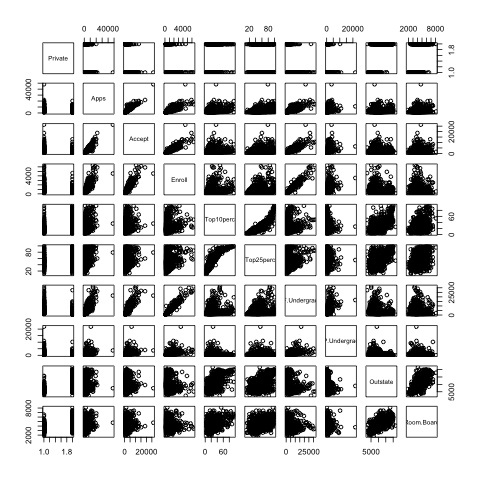
\includegraphics[width=.48\textwidth]{partII}
        \caption{Part II}
    \end{figure}

    \begin{figure}[h!]
        \centering
        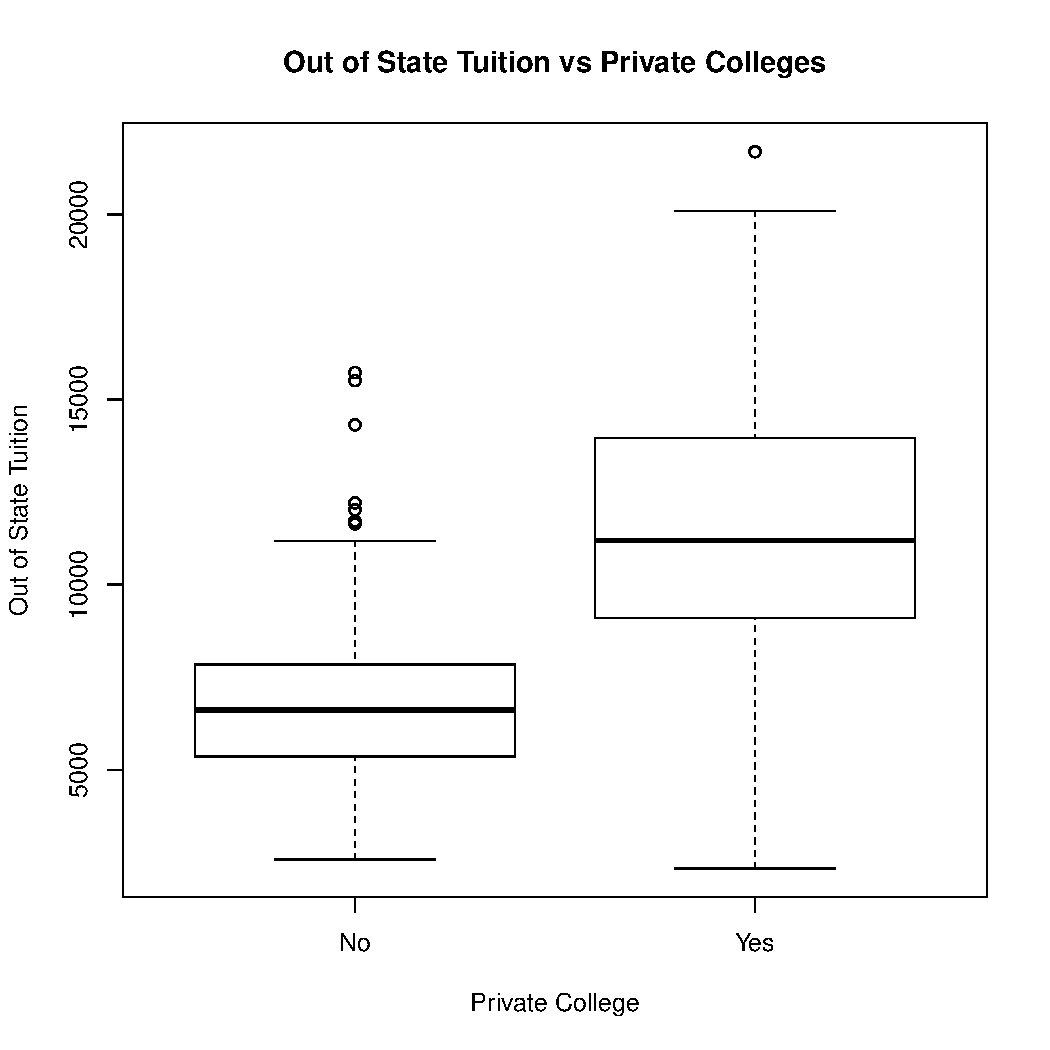
\includegraphics[width=.48\textwidth]{partIII}
        \caption{Part III}
    \end{figure}

    \begin{figure}[h!]
        \centering
        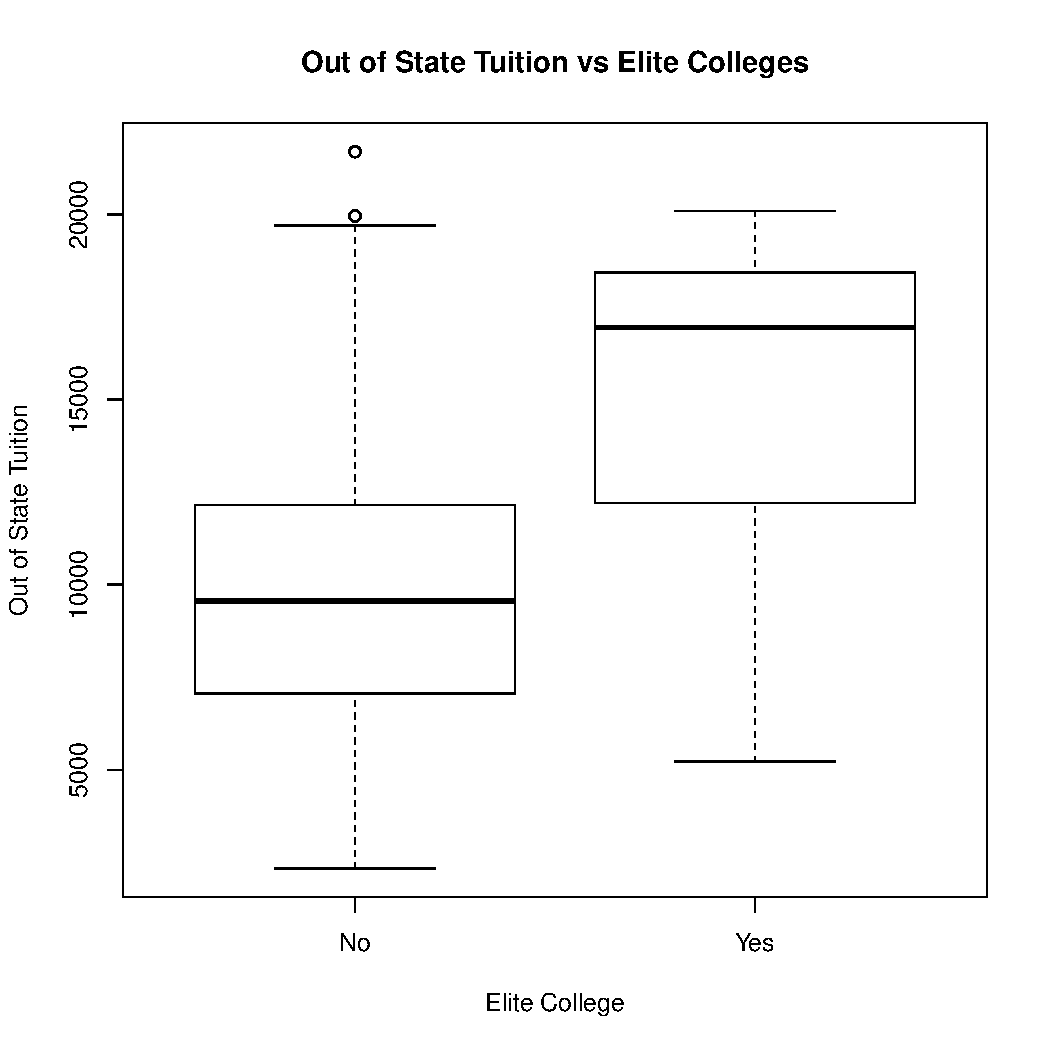
\includegraphics[width=.48\textwidth]{partIV}
        \caption{Part IV}
    \end{figure}

    \begin{figure}[h!]
        \centering
        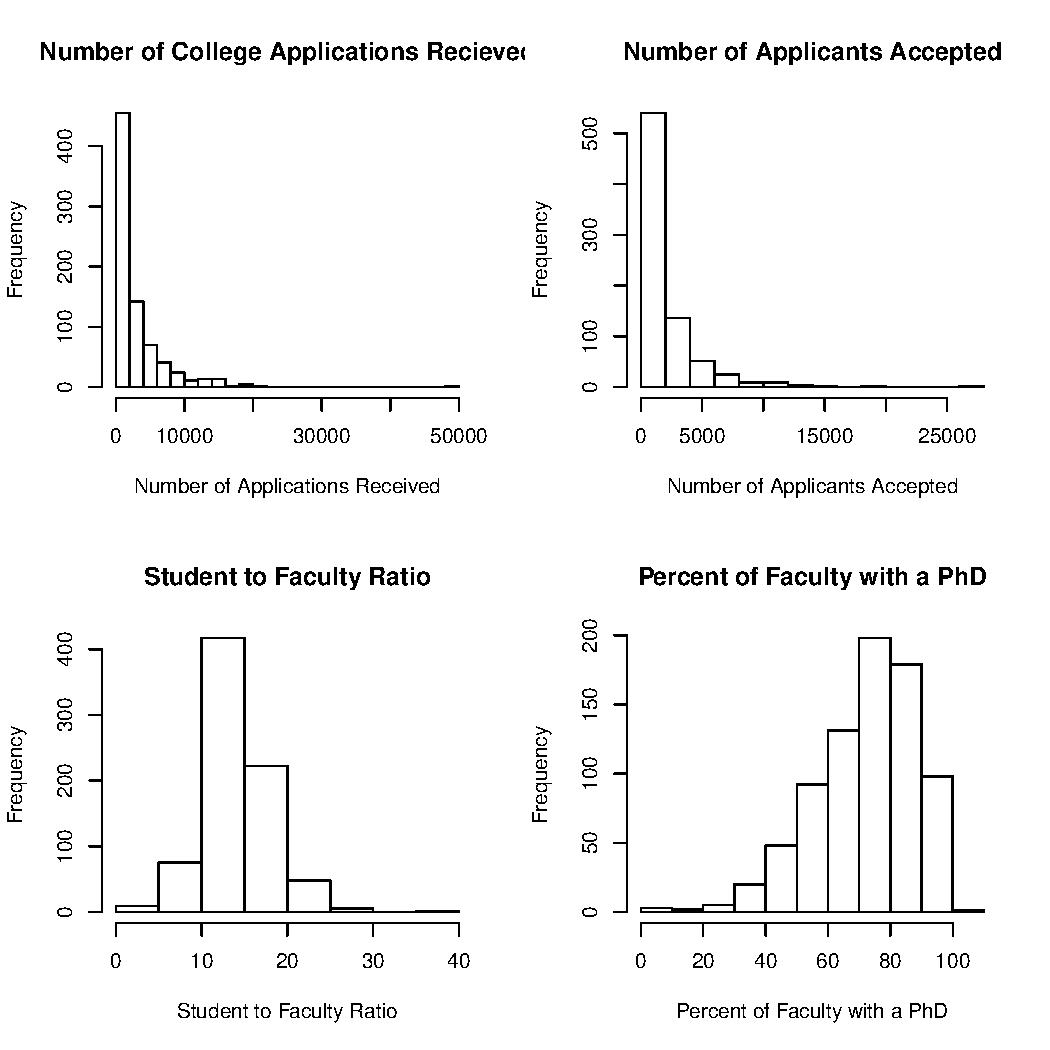
\includegraphics[width=.48\textwidth]{partV}
        \caption{Part V}
    \end{figure}
\end{homeworkProblem}

\pagebreak

\begin{homeworkProblem}
    Consider the following equation of a straight line \(Y_i = \beta_0 +
    \beta_1 x_i + e_i\) with \(i = 1, \ldots, n\), \(\E[e_i] = 0\), \(\Var[e_i]
    = \sigma^2_e\), and \(\Cov[e_i, e_j] = 0, \forall i \neq j\).
    \\

    \part

    Calculate the bias for the estimator of the intercept \(\hat{\beta_0}\).
    \\

    \solution

    Solution
    \\

    \part

    Calculate the variance for the estimator of the intercept \(\hat{\beta_0}\).
    \\

    \solution

    Solution.
\end{homeworkProblem}

\end{document}
